% Diagrama de Despliegue UML — SmartSupply (estado 2026-09)
\documentclass[tikz, border=14pt]{standalone}
\usepackage[utf8]{inputenc}
\usepackage[T1]{fontenc}
\usepackage{helvet}
\renewcommand{\familydefault}{\sfdefault}
\usetikzlibrary{positioning, arrows.meta, fit, backgrounds, calc}

\tikzset{
  art/.style={draw, line width=0.6pt, fill=white, align=left, anchor=north west,
    text width=#1, inner sep=5pt, font=\footnotesize\sffamily,
    path picture={
      \draw[line width=0.5pt]
        ([xshift=-0.36cm, yshift=-0.08cm]path picture bounding box.north east)
        -- ++(0.20,0) -- ++(0.08,-0.08) -- ++(0,-0.26) -- ++(-0.28,0) -- cycle;
    }},
  art/.default=4.0cm,
  dep/.style={line width=0.8pt, dashed, -{Latex[length=2.3mm]}},
  lbl/.style={font=\scriptsize\sffamily, fill=white, inner sep=1.2pt, align=center},
}
\newcommand{\at}{{\scriptsize\itshape\textless\textless artifact\textgreater\textgreater}\\}

% Nodo UML 3D alrededor de los artefactos: \dnode{id}{estereotipo}{nombre}{lista fit}
\newcommand{\dnode}[4]{%
  \begin{scope}[on background layer]
    \node[draw, line width=0.8pt, fill=white, inner xsep=10pt, inner ysep=8pt, fit=#4] (#1) {};
    \fill[white, draw=black, line width=0.8pt] (#1.north west) -- ++(0.3,0.3)
      -- ($(#1.north east)+(0.3,0.3)$) -- (#1.north east) -- cycle;
    \fill[black!12, draw=black, line width=0.8pt] (#1.north east) -- ++(0.3,0.3)
      -- ($(#1.south east)+(0.3,0.3)$) -- (#1.south east) -- cycle;
  \end{scope}
  \node[anchor=north west, align=left, font=\small\sffamily, inner sep=5pt] at (#1.north west)
    {{\scriptsize\itshape\textless\textless #2\textgreater\textgreater}\\\underline{#3}};
}

\begin{document}
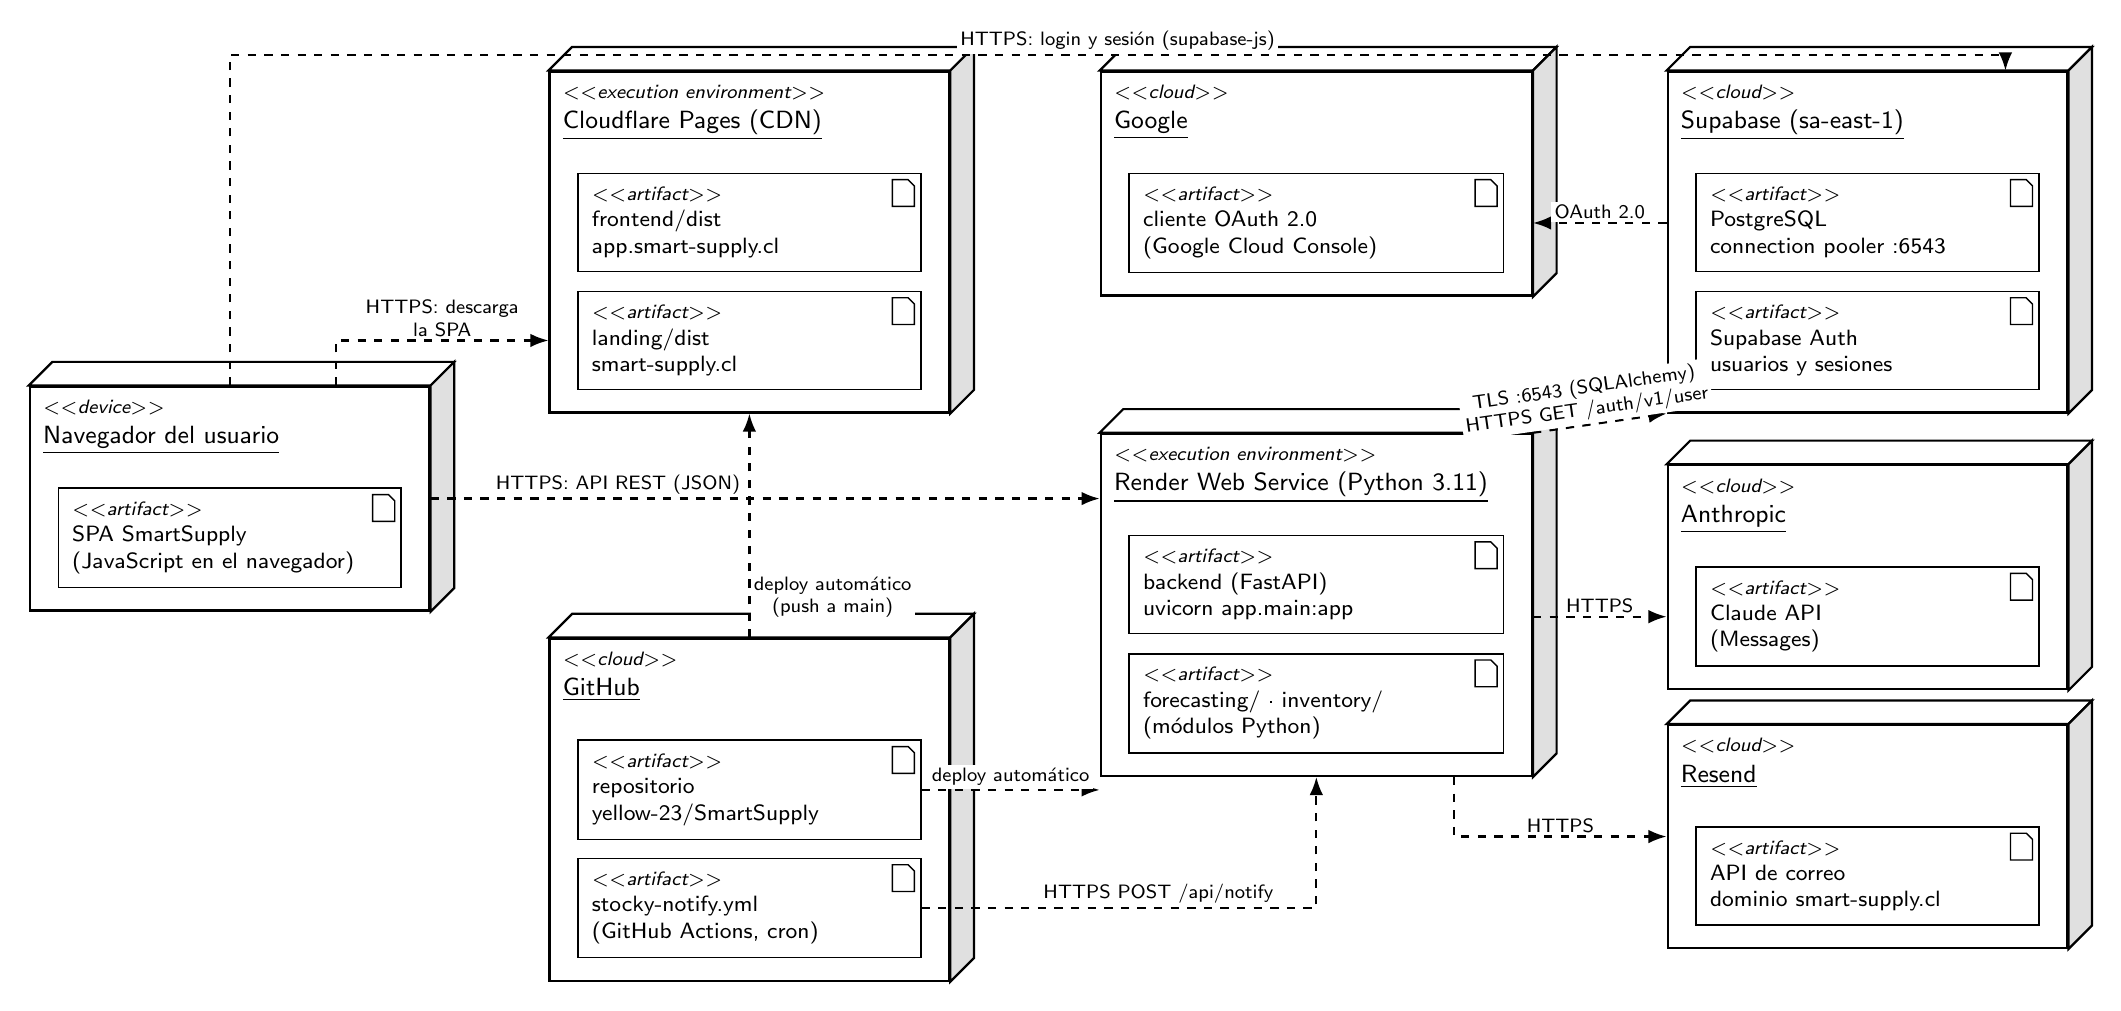
\begin{tikzpicture}[font=\sffamily]

% ── Navegador del usuario ───────────────────────────────────
\node[art=4.0cm] (nav1) at (-0.6, -4.0) {\at SPA SmartSupply\\ (JavaScript en el navegador)};
\coordinate (navT) at ($(nav1.north west)+(0,1.0)$);
\dnode{nav}{device}{Navegador del usuario}{(navT)(nav1)}

% ── Cloudflare Pages ────────────────────────────────────────
\node[art] (cf1) at (6.0, 0) {\at frontend/dist\\ app.smart-supply.cl};
\node[art] (cf2) at (6.0, -1.5) {\at landing/dist\\ smart-supply.cl};
\coordinate (cfT) at ($(cf1.north west)+(0,1.0)$);
\dnode{cf}{execution environment}{Cloudflare Pages (CDN)}{(cfT)(cf1)(cf2)}

% ── GitHub ──────────────────────────────────────────────────
\node[art] (gh1) at (6.0, -7.2) {\at repositorio\\ yellow-23/SmartSupply};
\node[art] (gh2) at (6.0, -8.7) {\at stocky-notify.yml\\ (GitHub Actions, cron)};
\coordinate (ghT) at ($(gh1.north west)+(0,1.0)$);
\dnode{gh}{cloud}{GitHub}{(ghT)(gh1)(gh2)}

% ── Render ──────────────────────────────────────────────────
\node[art=4.4cm] (r1) at (13.0, -4.6) {\at backend (FastAPI)\\ uvicorn app.main:app};
\node[art=4.4cm] (r2) at (13.0, -6.1) {\at forecasting/ · inventory/\\ (módulos Python)};
\coordinate (rT) at ($(r1.north west)+(0,1.0)$);
\dnode{rd}{execution environment}{Render Web Service (Python 3.11)}{(rT)(r1)(r2)}

% ── Google ──────────────────────────────────────────────────
\node[art=4.4cm] (g1) at (13.0, 0) {\at cliente OAuth 2.0\\ (Google Cloud Console)};
\coordinate (gT) at ($(g1.north west)+(0,1.0)$);
\dnode{go}{cloud}{Google}{(gT)(g1)}

% ── Supabase ────────────────────────────────────────────────
\node[art] (s1) at (20.2, 0) {\at PostgreSQL\\ connection pooler :6543};
\node[art] (s2) at (20.2, -1.5) {\at Supabase Auth\\ usuarios y sesiones};
\coordinate (sT) at ($(s1.north west)+(0,1.0)$);
\dnode{sb}{cloud}{Supabase (sa-east-1)}{(sT)(s1)(s2)}

% ── Anthropic y Resend ──────────────────────────────────────
\node[art] (a1) at (20.2, -5.0) {\at Claude API\\ (Messages)};
\coordinate (aT) at ($(a1.north west)+(0,1.0)$);
\dnode{an}{cloud}{Anthropic}{(aT)(a1)}

\node[art] (re1) at (20.2, -8.3) {\at API de correo\\ dominio smart-supply.cl};
\coordinate (reT) at ($(re1.north west)+(0,1.0)$);
\dnode{rs}{cloud}{Resend}{(reT)(re1)}

% ── Comunicaciones ──────────────────────────────────────────
\draw[dep] ([xshift=-12mm]nav.north east) |- (cf.west |- cf2.west) node[pos=0.75, lbl, above] {HTTPS: descarga\\la SPA};
\draw[dep] (nav.east) -- (rd.west |- nav.east) node[pos=0.28, lbl, above] {HTTPS: API REST (JSON)};
\draw[dep] (nav.north) -- ++(0,4.2) -| ([xshift=-8mm]sb.north east) node[pos=0.25, lbl, above] {HTTPS: login y sesión (supabase-js)};
\draw[dep] (sb.west |- g1.east) -- (go.east |- g1.east) node[midway, lbl, above] {OAuth 2.0};

\draw[dep] (rd.north east) -- (sb.south west) node[pos=0.42, lbl, sloped, above] {TLS :6543 (SQLAlchemy)\\HTTPS GET /auth/v1/user};
\draw[dep] (rd.east |- a1.west) -- (an.west |- a1.west) node[midway, lbl, above] {HTTPS};
\draw[dep] ([xshift=-10mm]rd.south east) |- (rs.west) node[pos=0.75, lbl, above] {HTTPS};

\draw[dep] (gh.north) -- (cf.south) node[pos=0.18, lbl, right] {deploy automático\\(push a main)};
\draw[dep] (gh1.east) -- (rd.west |- gh1.east) node[midway, lbl, above] {deploy automático};
\draw[dep] (gh2.east) -| (rd.south) node[pos=0.3, lbl, above] {HTTPS POST /api/notify};

\end{tikzpicture}
\end{document}
